\graphicspath{{1complex/asy/}}
\thispagestyle{empty}

\title{Math 147 --- Complex Analysis}
\author{Neil Donaldson}
\date{\today}
\maketitle	

\section{Complex Numbers}\label{chap:complex}

\subsection[Definition \& Basic Algebra]{Definition and Basic Algebraic Properties}
%Corresponds roughly to \S\,1--6 of the textbook: \emph{Complex Analysis and Applications}, James Ward Brown \& Ruel V.\ Churchill, 9th Ed 2014, McGraw Hill.}

In the 1500s, Italian mathematician Rafael Bombelli posited a solution to the seemingly absurd equation $x^2=-1$. By supposing that this solution behaved according to the usual rules of algebra, Bombelli and others were able to describe the solutions of any quadratic equation. To some extent, this was math for its own sake; Bombelli always considered his solutions to be entirely `fictitious.'\medbreak

For a modern definition, we start with the Cartesian plane $\R^2=\bigl\{(x,y):x,y\in\R\bigr\}$.

\begin{defn}{}{c}
	Given real numbers $\textcolor{red}{x},\textcolor{blue}{y}$, the \emph{complex number} $z=\textcolor{red}{x}+i\textcolor{blue}{y}$ is the point with co-ordinates $(\textcolor{red}{x},\textcolor{blue}{y})\in\R^2$. Its \emph{real} and \emph{imaginary parts} are the individual co-ordinates\par
	\begin{minipage}[t]{0.7\linewidth}\vspace{-15pt}
		\[
			\Re z=\textcolor{red}{x},\qquad \Im z=\textcolor{blue}{y}
		\]
		The \emph{complex numbers} $\C$ comprise the \emph{real} vector space $\R^2$ with the extra operation of \emph{complex multiplication}: if $z=\textcolor{red}{x}+i\textcolor{blue}{y}$ and $w=\textcolor{Green}{u}+i\textcolor{purple}{v}$, define
		\begin{itemize}
		  \item[](Vector) Addition: \ $z+w:=(\textcolor{red}{x}+\textcolor{Green}{u})+i(\textcolor{blue}{y}+\textcolor{purple}{v})$
		  \item[]Complex multiplication: \ $zw:= (\textcolor{red}{x}\textcolor{Green}{u} - \textcolor{blue}{y}\textcolor{purple}{v}) + i(\textcolor{red}{x}\textcolor{purple}{v} + \textcolor{blue}{y}\textcolor{Green}{u})$
		\end{itemize}
		When drawn with axes, the complex plane is known as the \emph{Argand diagram} and we refer, respectively, to the \emph{real} and \emph{imaginary axes.}
	\end{minipage}
	\hfill
	\begin{minipage}[t]{0.29\linewidth}\vspace{-15pt}
		\flushright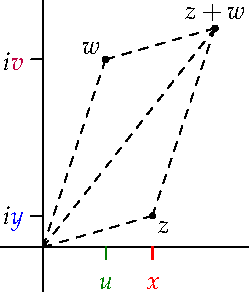
\includegraphics{intro-add}
	\end{minipage}
\end{defn}

Since $\C=\R^2$ is a real vector space under addition, several properties are immediate:

\begin{lemm}{Basic properties of complex addition}{}
	\begin{itemize}\itemsep2pt
	  \item[]Associativity: \ $z_1+(z_2+z_3)=(z_1+z_2)+z_3$
	  \item[]Commutativity: \ $z+w=w+z$ \ (this is the parallelogram law illustrated in the picture)
	  \item[](Real) scalar multiplication: \ $\forall \lambda\in\R$, \ $\lambda(x+iy)=\lambda x+i\lambda y$
	  \item[]Additive inverse: \ $-z=-(x+iy)=(-x)+i(-y)=-x-iy$
	\end{itemize}
\end{lemm}

\begin{example}{}{}
	If $z=\textcolor{red}{3}+\textcolor{blue}{4}i$ and $w=\textcolor{Green}{2}-\textcolor{purple}{7}i$, then
	\[
		z-w=z+(-w) = \bigl(\textcolor{red}{3}-\textcolor{Green}{2}\bigr) + \bigl(\textcolor{blue}{4}-(-\textcolor{purple}{7})\bigr)i =1+11i
	\]
\end{example}

\goodbreak


The natural distance measure from $\R^2$ transfers to $\C$ (the complex numbers are a real metric space).

\begin{defn}[lower separated=false, sidebyside, sidebyside align=top seam, sidebyside gap=0pt, righthand width=0.28\linewidth]{}{modulus}
	The \emph{modulus} of a complex number $z=x+iy$ is the Euclidean distance of the point $(x,y)$ from the origin:
	\[
		\nm z:=\sqrt{x^2+y^2}
	\]
	In the picture, $z=1+\sqrt 3 i$ has modulus $\nm z=\sqrt{1+3}=2$.
	\tcblower
	\flushright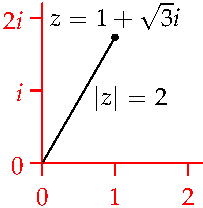
\includegraphics[scale=0.85]{intro-modulus}
\end{defn}


Some natural inequalities follow straight from the picture in Definition \ref{defn:c}.

\begin{lemm}{Triangle inequalities}{tri-ineq}
	For all $z,w\in\C$,
	\[
		\nm{z+w}\le \nm{z}+\nm{w}
		\quad\text{and}\quad
		\nm{z+w}\ge \bigl|\nm z-\nm w\bigr|
	\]
\end{lemm}

In the second (``extended") inequality, we take the \emph{absolute value} of the difference of the moduli. Unlike in $\R$, these inequalities relate to honest triangles! We can easily generalize the first by induction,
\[
	\nm{z_1+z_2+\cdots +z_n}\le\nm{z_1}+\cdots+\nm{z_n}
\]

The modulus may be used to describe various curves and regions in the plane. 

\begin{examples}[lower separated=false, sidebyside, sidebyside align=top seam, sidebyside gap=0pt, righthand width=0.3\linewidth]{}{}
	\exstart \textcolor{blue}{$\nm z=3$} describes the circle with radius 3 centered at the origin. In Cartesian co-ordinates, this is $x^2+y^2=9$.
	\begin{enumerate}\setcounter{enumi}{1}
	  \item \textcolor{Green}{$\nm{z-2-3i}\le 2$} describes the \emph{disk} with radius 2 centered at $2+3i$.
	  \item \textcolor{orange}{$\nm z+\nm{z-2}=4$} describes an \emph{ellipse} with foci 0 and 2. This is more familiar after multiplying out (try it!):
	  \begin{align*}
		  \sqrt{x^2+y^2}+\sqrt{(x-2)^2+y^2}=4 \implies
		  	&
		  (x-2)^2+y^2=\cdots\\%\left(4-\sqrt{x^2+y^2}\right)^2=\cdots%\\
		  \implies &\frac{(x-1)^2}4+\frac{y^2}3=1
	  \end{align*}
	\end{enumerate}
	\tcblower
	\flushright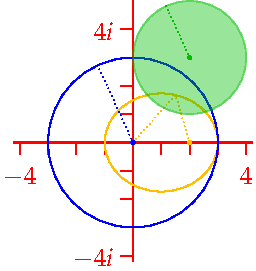
\includegraphics{intro-modulus3}
\end{examples}





\boldsubsubsection{Complex multiplication, division and the complex conjugate}

Multiplication is what really distinguishes the complex numbers from $\R^2$, and lead to all the interesting structure in this course. For starters, we instantly see that $i$ is a solution to Bombelli's absurd equation:
\[
	\tcbhighmath{i^2=(0+1i)(0+1i)=(0\cdot 0-1\cdot 1)+i(0\cdot 1+1\cdot 0)=-1}
\]


The upshot is that we can treat complex addition, subtraction and multiplication as if we are working with \emph{linear polynomials}\footnote{This is precisely the definition encountered in a Rings \&\ Fields course: $\C$ is the \emph{factor ring} of real polynomials modulo the \emph{ideal} $\ip{x^2+1}$.} in the abstract variable $i$; simply replace $i^2$ with $-1$ when needed.
 
\begin{example}{}{}
	If $z=\textcolor{red}{3}+\textcolor{blue}{4}i$ and $w=\textcolor{Green}{2}-\textcolor{purple}{7}i$, then
	\begin{align*}
		zw
		&= (\textcolor{red}{3}+\textcolor{blue}{4}i) (\textcolor{Green}{2}-\textcolor{purple}{7}i) = \textcolor{red}{3}\cdot \textcolor{Green}{2} + \textcolor{blue}{4}i\cdot \textcolor{Green}{2} - \textcolor{red}{3}\cdot \textcolor{purple}{7}i - \textcolor{blue}{4}i\cdot \textcolor{purple}{7}i = 6+8i-21i-28i^2\\
		&= 6+8i-21i+28=34-13i
	\end{align*}
\end{example}


The basic algebraic properties of complex multiplication are straightforward, if tedious, to verify:

\begin{lemm}{Basic properties of multiplication}{basic}
	For any complex numbers $z_1,z_2,z_3$,
	\begin{itemize}\itemsep2pt
	  \item[]Associativity: \ $z_1(z_2z_3)=(z_1z_2)z_3$
	  \item[]Commutativity: \ $z_1z_2=z_2z_1$
	  \item[]Distributivity: \ $z_1(z_2+z_3)=z_1z_2+z_1z_3$
	\end{itemize}
\end{lemm}

To develop division, it is is helpful to introduce a new concept.

\begin{defn}{}{}
	The \emph{(complex) conjugate} of $z=x+iy$ is $\cl z:=x-iy$ (``$z$-bar''). Geometrically, $\cl z$ is  obtained by reflection in the real axis.
\end{defn}

Observe that $z\cl z=(x+iy)(x-iy)=x^2+y^2=\nm z^2$, from which:

\begin{lemm}{}{}
	Every non-zero complex number $z=x+iy$ has a unique multiplicative inverse
	\[
		z^{-1}=\frac{\cl z}{\nm z^2}=\frac{x-iy}{x^2+y^2} \quad\text{satisfies}\quad zz^{-1}=1
	\]
\end{lemm}

\begin{proof}
	That $zz^{-1}=1$ is trivial. For uniqueness, suppose we also have $zw=1$; now use associativity and commutativity to conclude that
	\[
		w=(z^{-1}z)w=z^{-1}(zw)=z^{-1}\tag*{\qedhere}
	\]
\end{proof}

Division is simply multiplication by an inverse.

\begin{example}{}{}
	Given $z=\textcolor{red}{3}+\textcolor{blue}{4}i$ and $w=\textcolor{Green}{2}-\textcolor{purple}{7}i$, compute
	\begin{align*}
		\frac wz
		&= \frac{\textcolor{Green}{2} - \textcolor{purple}{7}i}{\textcolor{red}{3} + \textcolor{blue}{4}i}
		= wz^{-1}
		= \frac{w\cl z}{\nm z^2} 
		= \frac{(\textcolor{Green}{2} - \textcolor{purple}{7}i)(\textcolor{red}{3} - \textcolor{blue}{4}i)}{\nm{\textcolor{red}{3} + \textcolor{blue}{4}i}^2}
		= \frac{\textcolor{Green}{2} \cdot \textcolor{red}{3} - \textcolor{Green}{2} \cdot \textcolor{blue}{4}i - \textcolor{purple}{7}i \cdot \textcolor{red}{3} + \textcolor{purple}{7}i \cdot \textcolor{blue}{4}i}{\textcolor{red}{3}^2 + \textcolor{blue}{4}^2}\\
		&= \frac{6-8i-21i+28i^2}{25}
		= \frac{-22-29i}{25}
	\end{align*}
	Alternatively, we could multiply numerator and denominator by the conjugate\footnotemark{} of the denominator:
	\[
		\frac{\textcolor{Green}{2} - \textcolor{purple}{7}i}{\textcolor{red}{3} + \textcolor{blue}{4}i}
		= \frac{\textcolor{Green}{2} - \textcolor{purple}{7}i}{\textcolor{red}{3} + \textcolor{blue}{4}i} \cdot \frac{\textcolor{red}{3} - \textcolor{blue}{4}i}{\textcolor{red}{3} - \textcolor{blue}{4}i}
		= \cdots
	\]
\end{example}

\footnotetext{Compare this approach to elementary algebra where, for instance, we use the \emph{conjugate} $5+\sqrt 3$ of $5-\sqrt 3$ to evaluate the reciprocal $\frac 1{5-\sqrt 3}=\frac{5+\sqrt 3}{(5-\sqrt 3)(5+\sqrt 3)}=\frac{5+\sqrt 3}{22}$.}


This initial section \emph{should} be revision, though some unfamiliarity with terminology is expected. The goal at this stage is to be fluent when \emph{computing} with complex numbers. The exercises should feel straightforward, particularly 1--6; if not, ask for help! 

\begin{exercises}
	\exstart The real number 2 is also a complex number. What is it in co-ordinate form $(x,y)$? What about the complex number $i$?
	\begin{enumerate}\setcounter{enumi}{1}
	  \item For any $z\in\C$, prove that $\Re(iz)=-\Im z$ and that $\Im(iz)=\Re z$.
	  
	  \item\begin{enumerate}
	    \item Check that both $z=2+3i$ and its conjugate $\cl z=2-3i$ solve the quadratic equation $z^2-4z+13=0$.
	    \item More generally, suppose $a,b,c\in\R$ where $\omega:=4ac-b^2>0$. Verify that $z=\frac{-b+i\sqrt \omega}{2a}$ and its conjugate $\cl z$ both solve\footnotemark{} the quadratic equation $az^2+bz+c=0$.\par
	    
	  \end{enumerate}
	
	  \item Prove the commutativity of complex multiplication (Lemma \ref{lemm:basic}) using Definition \ref{defn:c}.
	  
	  \item Evaluate the following in the form $x+iy$.
	  \begin{enumerate}
	    \item $\dfrac{2-i}{3-5i}$\qquad (b)\ \ $(1+i)^4$\qquad (c)\ \ $(2+3i)^{-2}-(2-3i)^{-2}$
	  \end{enumerate}
	  
	  \item Prove the following. Write $z=x+iy$ rather than using the vector definition.
	  \begin{enumerate}
	    \item $\cl{\cl z}=z$\qquad (b)\ \ $(z^{-1})^{-1}=z$\qquad (c)\ \ $\cl{zw}=\cl z\cdot \cl w$
	  \end{enumerate}
	  
	  \item\label{ex:triangmod}\begin{enumerate}
	    \item Use the first version of the triangle inequality (Lemma \ref{lemm:tri-ineq}) to prove the second: for any $z,w\in\C$, we have $\displaystyle \nm{z+w}\ge \bigl|\nm z-\nm w\bigr|$.
	    \item What relationship between $z,w$ corresponds to \emph{equality} here? Draw a picture!
	  \end{enumerate}
	  
	  \item Suppose that $\nm z\ge 2$ and consider the polynomial $P(z)=z^3+3z-1$.
	  \begin{enumerate}
	    \item Use the triangle inequality to prove that $\nm{\frac{3z-1}{z^3}}\le\frac 78$
	    \item Write $\nm{P(z)}=\nm{z^3+3z-1}=\nm{z^3}\nm{1+\frac{3z-1}{z^3}}$. Now use the extended triangle inequality to prove that $\nm{P(z)}\ge 1$.\par
	    (\emph{This shows that all zeros of $P(z)$ lie inside the circle $\nm z<2$})
		\end{enumerate}
		
	 	\item By considering the inequality $(\nm x-\nm y)^2\ge 0$, prove that
	 	\[
	 		\sqrt 2\nm z\ge \nm{\Re z}+\nm{\Im z} \quad\text{for any}\quad z\in\C
	 	\]
	 	
	 	\item Prove that the hyperbola $x^2-y^2=1$ can be written in the form $z^2+\cl z^2=2$.
	 	 
	  \item Draw a picture of the ellipse satisfying the equation $\nm{z}+\nm{z-4i}=6$. Find the equation of the curve in Cartesian coordinates: $\frac{(x-c)^2}{a^2}+\frac{(y-d)^2}{b^2}=1$ where $(c,d)$ is the center of the ellipse and $a,b$ are its semi-axes.\par
	  (\emph{Hint: write $\nm{z-4i}=6-\nm z$, square both sides, cancel $x^2,y^2$ terms and repeat\ldots})
	\end{enumerate}
\end{exercises}

\footnotetext{Since $i^2=-1$, we may write $i\sqrt\omega =\sqrt{-\omega}$, whence the quadratic formula applies to all real quadratic equations!}

\clearpage



\subsection[The Polar Form]{The Exponential/Polar Form of a Complex Number}
%(\S\,7--9)

\begin{defn}[lower separated=false, sidebyside, sidebyside align=top seam, sidebyside gap=0pt, righthand width=0.25\linewidth]{}{argument}
	A complex number can be written in polar co-ordinates:
	\[
		z=x+iy =r\cos\theta+ir\sin\theta =r(\cos\theta+i\sin\theta)
	\]
	Plainly $r=\nm z$ is the modulus. We call the angle $\theta=\arg z$ the \emph{argument} of $z$.\smallbreak
	The argument is \emph{multi-valued} in the sense that $\arg z=\theta+2\pi n$ for any integer $n$. For clarity, we distinguish the \emph{principal argument} $\Arg z$ by insisting that $-\pi<\Arg z\le \pi$.
	\tcblower
	\flushright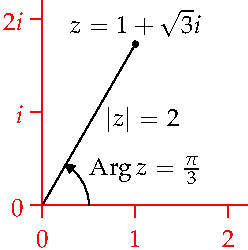
\includegraphics[scale=0.9]{intro-modulus2}
\end{defn}

Note that 0 has no argument; it is the only such complex number.

\begin{example}{}{}
	In the above picture, $z=1+\sqrt 3 i$ has principal argument $\Arg z=\frac\pi 3$. You can write the argument either as many different values, or as a set:\footnotemark{} the following are all legitimate
	\[
		\arg z=\{\tfrac\pi 3+2\pi n:n\in\Z\}\quad\text{or}\quad \arg z=\tfrac\pi 3\quad\text{or}\quad \arg z=\tfrac{7\pi}3
	\]
\end{example}

\footnotetext{This is merely the common mathematical fudge of replacing an equivalence class $\{\tfrac\pi 3+2\pi n:n\in\Z\}$ by any of its representatives, e.g.\ $\frac\pi 3$ or $\frac{7\pi}3$.}

If $x\neq 0$, is it almost trivial to compute the argument:
\[
	\begin{cases}
		x=r\cos\theta\\
		y=r\sin\theta
	\end{cases}
	\negthickspace\negthickspace\negthickspace
	\implies \tan\theta=\frac yx \overset{\text{???}}{\implies} \Arg z=\tan^{-1}\frac yx
\]

\begin{minipage}[t]{0.55\linewidth}\vspace{0pt}
	This isn't quite right. Since $\arctan$ has range $(-\frac\pi 2,\frac\pi 2)$, an addition or subtraction of $\pi$ is required to find the correct value whenever $z$ lies in the second or third quadrants.
	
	\begin{example}{}{}
		Since $z=-3-3i$ lies in the third quadrant, we have
		\[
			\Arg z=\textcolor{Green}{\tan^{-1}\frac{-3}{-3}-\pi}=-\frac{3\pi}4
		\]
		If we wanted the argument to be positive, we could choose a non-principal argument $\arg z=\frac{5\pi}4$.
	\end{example}
\end{minipage}
\hfill
\begin{minipage}[t]{0.44\linewidth}\vspace{-50pt}
	\flushright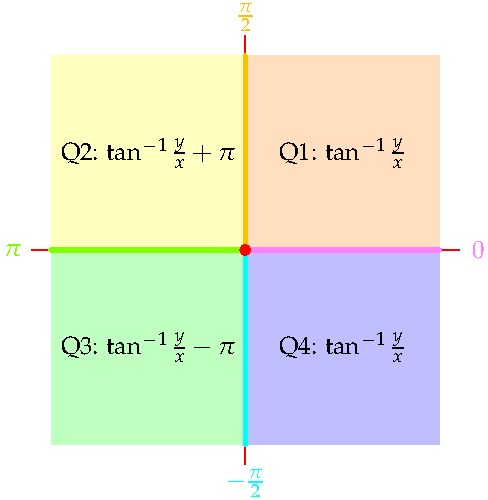
\includegraphics[scale=0.9]{intro-argument}
\end{minipage}
\bigbreak

The polar form allows us to define a crucial new function.

\begin{defn}{}{}
	Given $\theta\in\R$, the \emph{complex exponential} $e^{i\theta}$ is defined by \emph{Euler's formula}
	\[
		e^{i\theta}:=\cos\theta+i\sin\theta
	\]
	The \emph{polar form} of a complex number is $z=re^{i\theta}$ where $r=\nm z$ and $\theta=\arg z$ (\emph{any} argument! why?).\smallbreak
	If $w=u+iv$ is complex, then its exponential is defined by $e^w:=e^ue^{iv}=e^u(\cos v+i\sin v)$.
\end{defn}
\goodbreak


Euler's formula provides a sensible definition of $e^{i\theta}$ since it fits with two common definitions of the exponential in real analysis.
\begin{enumerate}
  \item If $k\in\R$, then $e^{k\theta}$ is the solution to the initial value problem $y'=ky$ with $y(0)=1$. Assuming that differentiation works when $k=i$, Euler's formula also satisfies this criterion:
  \[
  	\diff\theta e^{i\theta} = \diff\theta(\cos\theta+i\sin\theta) = -\sin\theta+i\cos\theta=i(\cos\theta+i\sin\theta) = ie^{i\theta} 
  \]
	\item The real and imaginary parts of the Maclaurin series $\exp z=\sum\frac{z^n}{n!}$ evaluated at $z=i\theta$ are, respectively, the Maclaurin series of $\cos\theta$ and $\sin\theta$.
\end{enumerate}

A third reason is that the definition satisfies the usual exponential laws.

\begin{lemm}{Exponential laws}{explaws}
	Let $z=re^{i\theta}$ and $w=se^{i\psi}$ be written in polar form. Then:
	\begin{enumerate}
	  \item $zw=rse^{i(\theta+\psi)}$. In particular, $\nm{zw}=\nm z\nm w$ and $\arg zw=\arg z+\arg w$
	  \item $\frac zw=\frac rse^{i(\theta-\psi)}$
	  \item $z^n=r^ne^{in\theta}$ for all $n\in\Z$
	\end{enumerate}
\end{lemm}

Note that the \emph{principal argument} might not behave so nicely for products; the best we can say is that
\[\tcbhighmath{\Arg zw=\Arg z+\Arg w+2\pi n\text{ for some }n=0,\pm 1}\]

\begin{proof}
Part 1 follows from the multiple-angle formulæ for sine and cosine:
\begin{align*}
e^{i(\theta+\psi)}&=\cos(\theta+\psi)+i\sin(\theta+\psi) =\cos\theta\cos\psi-\sin\theta\sin\psi+ i(\sin\theta\cos\psi+\cos\theta\sin\psi)\\
&=(\cos\theta+i\sin\theta)(\cos\psi+i\sin\psi) =e^{i\theta}e^{i\psi}
\end{align*}
Parts 2 and 3 are now straightforward.
\end{proof}

\begin{examples}{}{argproduct}
	\exstart Given $z=-7+i$ and $w=3+4i$, we compute the modulus and argument of $zw$ in two ways:
	\begin{enumerate}\setcounter{enumi}{1}
	  \item[]\begin{enumerate}
	    \item\label{ex:argproduct1a} Find the polar forms of $z,w$ before applying the Lemma:
	  	\begin{gather*}
		  	z=\nm ze^{i\arg z} = 5\sqrt{2}\exp\left(i(\pi-\tan^{-1}\tfrac 17)\right),\quad w=\nm we^{i\arg w}=5\exp\left(i\tan^{-1}\tfrac 43\right)\\
		  	\implies\nm{zw}=\nm z\nm w = 25\sqrt{2},\quad \arg zw= \arg z+\arg w = \pi-\tan^{-1}\frac 17+\tan^{-1}\frac 43
	  	\end{gather*}
	  	\item Find $zw=(-7+i)(3+4i)=-25-25i$ then compute its polar form:
	  	\[
	  		zw=25\sqrt 2\polarn{3\pi i}4\implies \nm{zw}=25\sqrt 2,\qquad \Arg zw=-\frac{3\pi}4
	  	\]
			\end{enumerate}
			The first approach is certainly uglier! It is usually better to use the second approach unless the arguments of $z,w$ are easily computable. In Exercise \ref{ex:argproduct2}, we check that these values correspond.
		
		\item We compute $z^{10}$ when $z=\sqrt 3-i$. First observe that $z=2\polarn{\pi i}6$, from which
		\[
			z^{10}=2^{10}\polarn{5\pi i}3 =1024\polar{\pi i}3 =512(1+\sqrt 3i)
		\]
	
		\item The identity $(e^{i\theta})^n=e^{in\theta}$ ($n\in\Z$) is known as \emph{de Moivre's formula}. It is usually written
		\[
			\tcbhighmath{(\cos\theta+i\sin\theta)^n=\cos n\theta+i\sin n\theta}
		\]
		Many trigonometric identities follow by taking real/imaginary parts. For instance, when $n=3$,
		\begin{gather*}
			\cos 3\theta+i\sin 3\theta =(\cos\theta+i\sin\theta)^3 =\cos^3\!\theta+3i\cos^2\!\theta\sin\theta-3\cos\theta\sin^2\!\theta -i\sin^3\!\theta\\
			\implies \cos 3\theta=\cos^3\!\theta-3\cos\theta\sin^2\!\theta=4\cos^3\!\theta-3\cos\theta
		\end{gather*}
	\end{enumerate}
\end{examples}

As before, this shouldn't be difficult. This section is merely polar co-ordinates in a different language!


\begin{exercises}
	\exstart Use induction to prove that for any $n\in\N_{\ge 2}$,
	\[
		e^{i\theta_1}e^{i\theta_2}\cdots e^{i\theta_n}=e^{i(\theta_1+\theta_2+\cdots+\theta_n)}
	\]

	\begin{enumerate}\setcounter{enumi}{1}
		\item Find the principal argument of $(1+i)^{2024}$.
		
		\item Prove that $\nm{e^{i\theta}}=1$ and that $\cl{e^{i\theta}}=e^{-i\theta}$.
	
		\item\begin{enumerate}
		  \item Show that if $\Re z>0$ and $\Re w>0$, then $\Arg zw=\Arg z+\Arg w$.
			\item If $z$ and $w$ both lie in quadrant 2, explain why $\Arg zw=\Arg z+\Arg w-2\pi$.
		\end{enumerate}
	
	 	\item Prove that non-zero $z,w\in\C$ have the same modulus if and only if $\exists p,q\in\C$ such that $z=pq$ and $w=p\cl q$.
		
	  \item\label{ex:deM} Use de Moivre's formula to establish the identity
	  \[
	  	\cos 4\theta=8\cos^4\!\theta-8\cos^2\!\theta+1
	  \]
	  
	  \item\label{ex:argproduct2}
	  \begin{enumerate}
	    \item Let $\alpha=\tan^{-1}\frac 43$ and $\beta=\tan^{-1}\frac 17$. Use right-triangles to show that
	  	\[
	  		\cos\alpha=\frac 35,\qquad\sin\alpha=\frac 45,\qquad\cos\beta=\frac 7{\sqrt{50}},\qquad\sin\beta=\frac 1{\sqrt{50}}
	  	\]
	  	Now use the cosine multiple-angle formula to check that $\alpha-\beta=\frac\pi 4$.\par
	  	(\emph{This shows that $\arg zw=\frac{5\pi}4$ in Example \ref{ex:argproduct}(a)})
	  	
	  	\item Generalize the approach in part (a): if $0<\beta<\alpha<\frac\pi 2$, prove the multiple-angle formula
	  	\[
	  		\tan(\alpha-\beta)=\frac{\tan\alpha-\tan\beta}{1+\tan\alpha\tan\beta}
	  	\]
	  \end{enumerate}
	  
	 
	  \item The polar form of a complex number is well-suited to describing \emph{circles.} For instance the circle centered at $i$ with radius 3 may be described by $z=i+3e^{i\theta}$ where $-\pi<\theta\le\pi$. 
	  \begin{enumerate}
	    \item Describe the circle centered at $z_0=3+4i$ with radius 2.
	    
	    \item Show that the points $z=re^{i\theta}$ for which $r=2a\cos\theta$ describe a circle.\par
	    (\emph{Hint: Multiply by $r$})	
		\end{enumerate}
	\end{enumerate}
\end{exercises}

\clearpage



\subsection{Roots of Complex Numbers}\label{sec:roots}% (\S\,10--11)

A naïve approach to taking roots in $\C$ is very messy.

\begin{example}{}{rootsimple}
	To find $c$ such that $c^2=-5+12i$, we need to solve an equation:
	\[
		-5+12i=c^2=(x+iy)^2=x^2-y^2+2ixy\iff 
		\begin{cases}
			x^2-y^2=-5\\
			xy=6
		\end{cases}
	\]
	Substituting $y=6x^{-1}$ into the first equation yields a quadratic in $x^2$:
	\[
		x^4+5x^2-36=(x^2-4)(x^2+9)
	\]
	We conclude that $x=\pm 2$, and obtain the square roots $\pm c=\pm(2+3i)$.
\end{example}

The example is reassuring in that we obtain precisely two square roots. Unfortunately, extending the method to cube, or higher, roots seems doomed! Instead we use the polar form. Suppose $n\in\N$ and that $c,z$ satisfy $z=c^n$. In polar form
\[
	z=re^{i\theta},\quad c=se^{i\psi}\implies re^{i\theta}=s^ne^{in\psi}
\]
By equating moduli and arguments, we see that
\[
	r=s^n,\qquad n\psi=\theta+2\pi k\tag{$\ast$}
\]
where $k$ is some integer. We'll shortly put this together to obtain a proper definition, but we already have enough for a calculation.

\begin{example}{}{}
	We compute the fifth roots of $z=2e^{\frac{2\pi i}3}=-1+i\sqrt 3$.\par
	\begin{minipage}[t]{0.65\linewidth}\vspace{-4pt}
		In the above language, $2=s^5$, whence
		\[
			s=\sqrt[5]{2},\quad \psi=\frac 15\left(\frac{2\pi}3+2\pi k\right)=\frac{2\pi}{15}(1+3k)
		\]
		which results in the fifth roots
		\begin{gather*}
			\makebox[260pt][s]{$c_0=\sqrt[5]{2}\polar{2\pi i}{15}\hfill
			c_1=\sqrt[5]{2}\polar{8\pi i}{15}\hfill
			c_2=\sqrt[5]{2}\polar{14\pi i}{15}$}\\[5pt]
			\makebox[260pt][s]{$c_3=\sqrt[5]{2}\polar{20\pi i}{15} =\sqrt[5]{2}\polarn{10\pi i}{15}\hfill
			c_4=\sqrt[5]{2}\polar{26\pi i}{15} =\sqrt[5]{2}\polarn{4\pi i}{15}$}
		\end{gather*}
		There are precisely \emph{five} fifth roots: once $k\ge 5$, the roots start repeating! The last two roots were written both with positive and principal arguments; both have their advantages.
	\end{minipage}
	\hfill
	\begin{minipage}[t]{0.34\linewidth}\vspace{-20pt}
		\flushright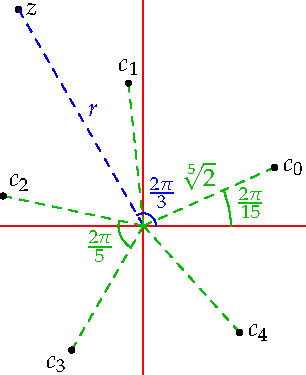
\includegraphics{intro-roots}
	\end{minipage}
	\medbreak
	Observe also how the fifth roots form the vertices of a regular pentagon, equally spaced around the circle of radius $\sqrt[5]{2}$. Is it obvious to you why this is so?\smallbreak
	Finally, note how essential the polar form was to this calculation. We could convert back to rectangular form, but since $\cos\frac{2\pi}{15}$ and $\sin\frac{2\pi}{15}$ are unfriendly values, there is little benefit. 
\end{example}


\goodbreak


\begin{defn}{}{nthroot}
	Given a non zero complex number $z=re^{i\theta}$ and a positive integer $n$, the \emph{$n\th$ roots} of $z$ are the $n$ distinct complex numbers
	\[
		c_k=\sqrt[n]{r}\exp\frac{(\theta+ 2k\pi)i}n\qquad k=0,1,\ldots,n-1
	\]
	where $\sqrt[n]{r}$ is the real (positive!) $n\th$ root of $r$.\smallbreak
	There are some conventions to follow. Let $\theta=\Arg z$ be the \emph{principal argument} of $z$:
	\begin{enumeratea}
	  \item The \emph{principal $n\th$ root} is written $\sqrt[n]{z}:=\sqrt[n]{r}\polar{i\theta}n$.
	  \item The \emph{set of $n\th$ roots} is denoted $z^{\frac 1n}:=\{c_0,\ldots,c_{n-1}\}$.
	\end{enumeratea}
	Denote by $\omega_n=\polar{2\pi i}n$ a \emph{primitive $n\th$ root of unity} ($n\th$ root of 1). Then the full set of \emph{$n\th$ roots of unity} is
	\[
		1^{\frac 1n}=\{\omega_n^k:k=0,\ldots,n-1\}=\{\polar{2\pi k i}n:k=0,\ldots,n-1\}
	\]
\end{defn}


The $n\th$ roots of $z$ may be written in terms of the principal root and the $n\th$ roots of unity
\[
	z^{\frac 1n}=\sqrt[n]{z}\,1^{\frac 1n}=\{\sqrt[n]{z}\omega_n^k:k=0,\ldots,n-1\}
\]
By the exponential laws (Lemma \ref{lemm:explaws}), multiplication by $\omega_n^k=\polar{2\pi ki}n$ has the geometric effect of rotating counter-clockwise by $\frac{2\pi k}n$ radians:
\[
	\arg\sqrt[n]z\omega_n^k=\arg\sqrt[n]z+\arg\omega_n^k=\arg\sqrt[n]z+\frac{2\pi k}n
\]
It follows that the $n\th$ roots of $z=re^{i\theta}$ form the vertices of a regular $n$-gon spaced equally round the circle of radius $\sqrt[n]{r}$. Compare this with the previous example.


\begin{examples}{}{}
	\exstart As a sanity check, we compare what happens when $n=4$ and $z=r=16$ is \emph{real} and \emph{positive.}
	\begin{enumerate}\setcounter{enumi}{1}
	  \item[]\begin{itemize}
		  \item The principal fourth root $\sqrt[4]{16}=2$ is the usual positive real fourth root.
		  \item Within the real numbers, we have \emph{two} fourth roots: $16^{\frac 14}=\pm 2$.
		  \item Within $\C$, there are \emph{four} fourth roots: $16^{\frac 14}=\{2,2i,-2,-2i\}$ where $i=\omega_4=\polar{i\pi}2$ is a primitive fourth root of unity.
	\end{itemize}
	
	  \item We compute the fourth roots of $z=8\sqrt 2(1+i)$.\smallbreak
		First we write in polar form: $z=16\polar{\pi i}4$. Since $\Arg z=\frac\pi 4$, the principal fourth root is
		\[
			\sqrt[4]{8\sqrt 2(1+i)}=2\polar{\pi i}{16}
		\]
		To find all fourth roots, simply multiply by the fourth roots of unity $1^{\frac 14}=\{1,i,-1,-i\}$:
		\[
			\left(8\sqrt 2(1+i)\right)^{\frac 14}=\{\pm 2\polar{\pi i}{16},\pm 2i\polar{\pi i}{16}\} =\{2\polar{\pi i}{16},2\polar{9\pi i}{16},2\polarn{15\pi i}{16},2\polarn{7\pi i}{16}\}
		\]
	 	Evaluating these in rectangular form is messy but doable (see Exercise \ref{ex:fourthrootrect}). In practice it is better to leave such expressions in polar form.	
	\end{enumerate}
\end{examples}


\goodbreak

The language of $n\th$ roots is likely less familiar, and will take more getting used to, than the material in the previous sections. With a little practice it is very easy, but fluency will take some investment of time.

\begin{exercises}
	\exstart Find the sixth roots of $i$ in polar co-ordinates. Which is the principal root?
	\begin{enumerate}\setcounter{enumi}{1}
  	\item Find the square roots of $-\sqrt 3+i$ and express them in rectangular co-ordinates.\par
  	(\emph{Hint: you may find the fact that $(\sqrt 3-1)^2=4-2\sqrt 3$ useful})
  
	  \item Use the fact that the cube roots of unity are $1,\omega_3=\frac{-1+\sqrt 3 i}2$ and $\omega_3^2=\frac{-1-\sqrt 3 i}2$ to evaluate the cube roots of $-27$ in rectangular co-ordinates.
	 
	  \item We previously found the fourth roots of 16. Use these to find the fourth roots of $-16$. Hence factorize the equation $z^4+16=0$ as a product of two quadratic equations with real coefficients.
	  
	  \item If $\omega$ is an $n\th$ root of unity \emph{other than 1,} prove that $\smash[b]{\sum\limits_{k=0}^{n-1}\omega^k=0}$.\par
	  (\emph{Hint: recall the geometric series formula})
	  
	  \item\begin{enumerate}
	    \item Suppose that $a,b,c\in\C$ with $a\neq 0$ and suppose that $z$ satisfies the quadratic equation $az^2+bz+c=0$. Prove the quadratic formula:
	    \[
	    	z=\frac{-b+(b^2-4ac)^{1/2}}{2a}
	    \]
	    Note that $(b^2-4ac)^{1/2}$ is the \emph{set} of square roots of $b^2-4ac$, so that this provides \emph{two} solutions whenever $b^2-4ac\neq 0$.
	    \item Find the roots of the equation $iz^2+(1+i)z+3=0$ in rectangular form.
	  \end{enumerate} 
	  
	  \item\label{ex:fourthrootrect} Use the half-angle formula $\cos^2\!\frac\alpha 2=\frac 12(1+\cos\alpha)$ to explicitly evaluate $\cos\frac\pi 8$ and then $\cos\frac\pi{16}$. Hence find an expression for the rectangular form of $\sqrt[4]{8\sqrt 2(1+i)}=2\polar{\pi i}{16}$ using only square roots.
	  
	  \item Recall Example \ref{ex:rootsimple}. Verify that the method in Definition \ref{defn:nthroot} gives the same value for the principal square root $\sqrt{-5+12i}$.\par
	  (\emph{You'll need some trig identities\ldots})
	
	\end{enumerate}
\end{exercises}